% numerical.tex

\cleardoublepage
\chapter{Ascent Trajectory}\label{chapter:numerical}


- keep this DIDO and hypaero and direct shooting

-explain why I moved to other GPOPS and CART3D at the end of the chapter


This chapter presents an optimised ascent trajectory of the three stage rocket-scramjet-rocket system. First the third stage trajectory optimised for maximum payload-to-orbit, and results tabulated for a range of second-third stage release points. Then, the second stage trajectory is optimised for maximum payload-to-orbit. The third stage payload-to-orbit database is used as the optimisation cost for the second stage, by interpolating for the release point obtained at the end of the trajectory. The first stage trajectory is optimised last. The first stage is optimised for the minimum fuel required to reach the first to second stage release point defined by the second stage optimal trajectory. The reason for using a different objective for the first stage is that the first stage mass defines the ability of the first stage to turn, as well as the amount that it can accelerate. If the first stage design is set, it will define much of the optimal trajectory for the second stage. 


\section{Third Stage trajectory}
-Details on methodology
-outline the limits that I put on it (ie cant go below starting altitude)
-I should maybe run a case without these limits to show the difference
-outline necessity for differing guess (will need to cite this as a regularly used process)
\begin{figure}
\centering
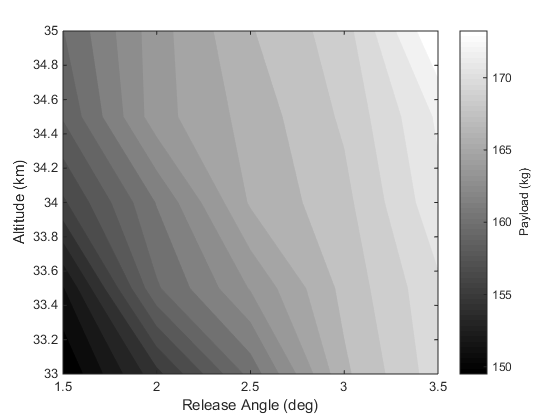
\includegraphics[width=0.7\linewidth]{figures/5_Ascent/contours}
\caption{}
\label{fig:contours}
\end{figure}

\begin{figure}
\centering
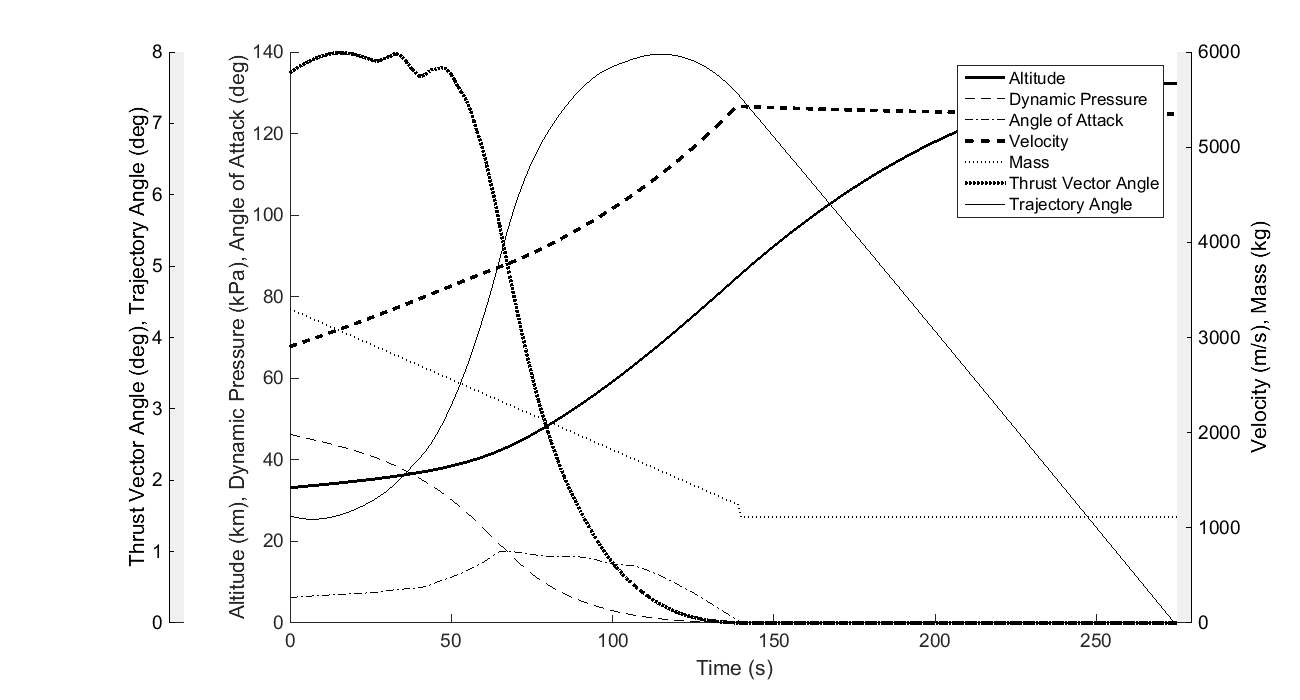
\includegraphics[width=0.9\linewidth]{figures/5_Ascent/ThirdStageConstQ}
\caption{}
\label{fig:ThirdStageConstQ}
\end{figure}
\begin{figure}
\centering
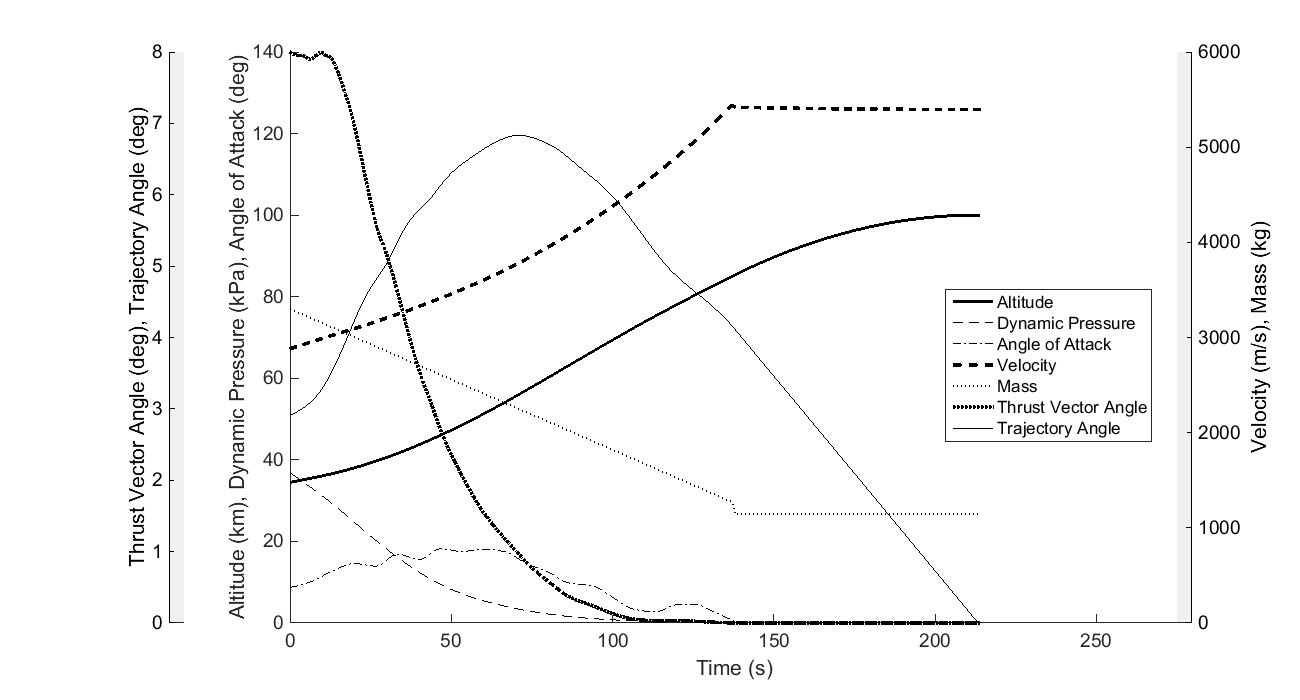
\includegraphics[width=0.9\linewidth]{figures/5_Ascent/ThirdStage50kpaconstrained}
\caption{}
\label{fig:ThirdStage50kpaconstrained}
\end{figure}



\section{SPARTAN trajectory}
-constant q
-45kPa,50kPa and 55kPa limited trajectories
-high drag trajectory

-it might be interesting to compare different third stage rocket engines 

\subsection{Constant Dynamic Pressure}
\begin{figure}
\centering
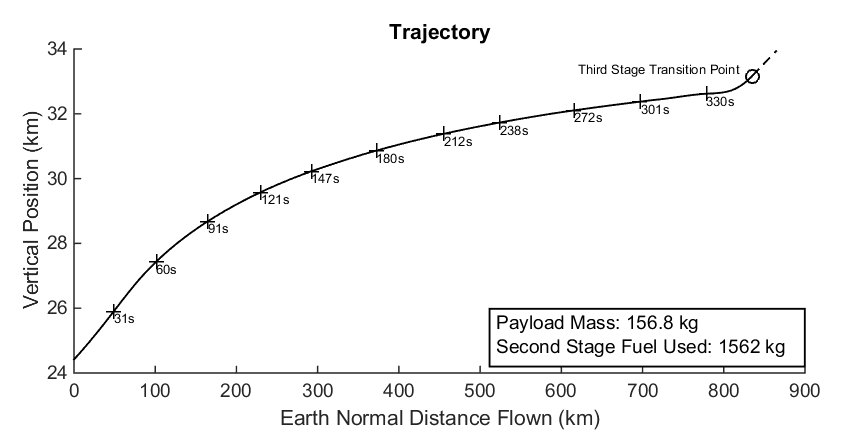
\includegraphics[width=0.9\linewidth]{figures/5_Ascent/Constq}
\caption{}
\label{fig:Constq}
\end{figure}
\begin{figure}
\centering
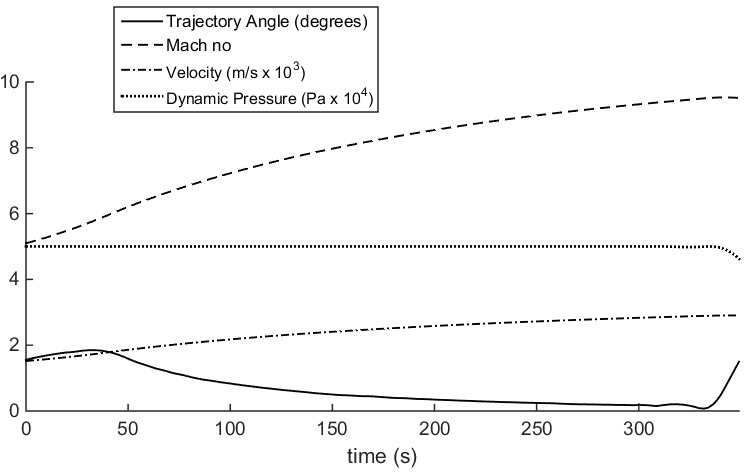
\includegraphics[width=0.8\linewidth]{figures/5_Ascent/Constq-Aero}
\caption{}
\label{fig:Constq-Aero}
\end{figure}
\begin{figure}
\centering
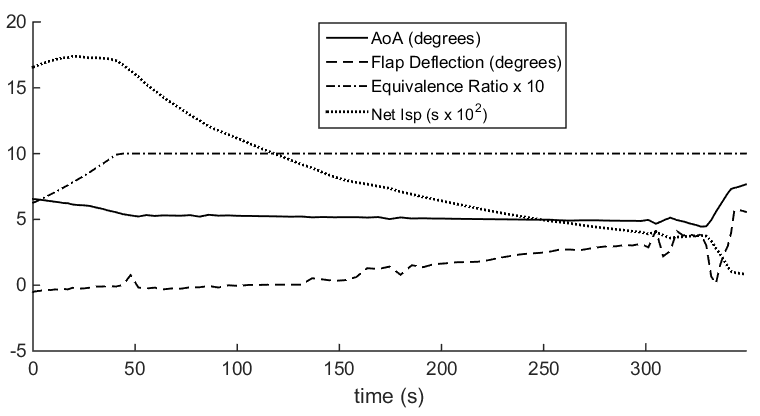
\includegraphics[width=0.8\linewidth]{figures/5_Ascent/Constq-Vehicle}
\caption{}
\label{fig:Constq-Vehicle}
\end{figure}

\subsubsection{Optimality Validation}


\subsection{Optimal Payload}
\begin{figure}
\centering
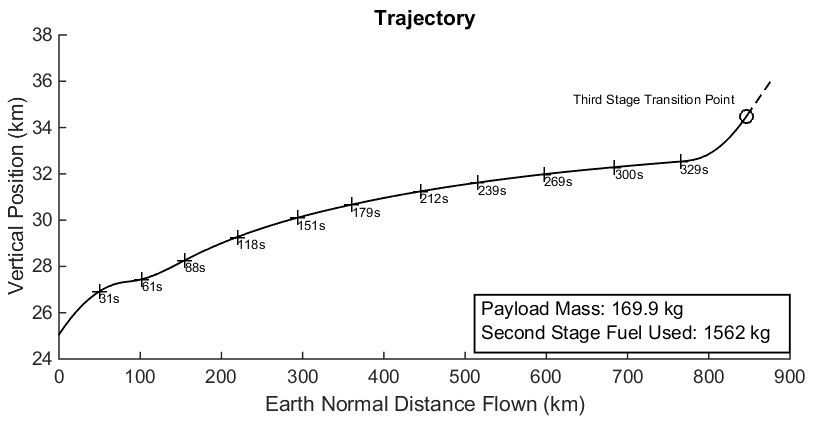
\includegraphics[width=0.9\linewidth]{figures/5_Ascent/qlimited50kpa}
\caption{}
\label{fig:qlimited50kpa}
\end{figure}
\begin{figure}
\centering
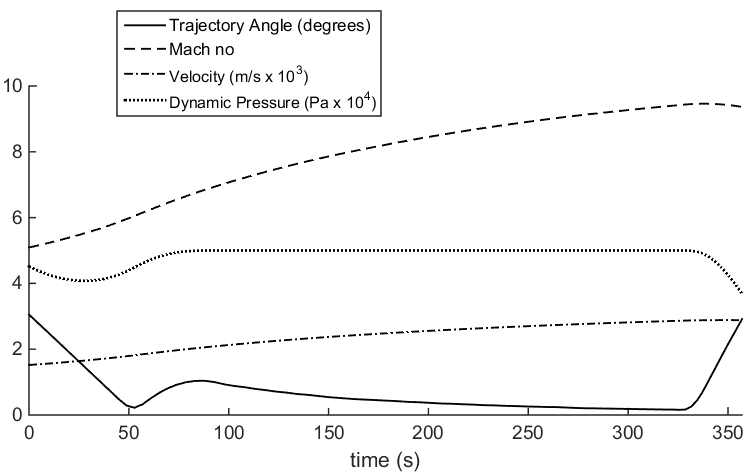
\includegraphics[width=0.8\linewidth]{figures/5_Ascent/qlimited50kpa-Aero}
\caption{}
\label{fig:qlimited50kpa-Aero}
\end{figure}
\begin{figure}
\centering
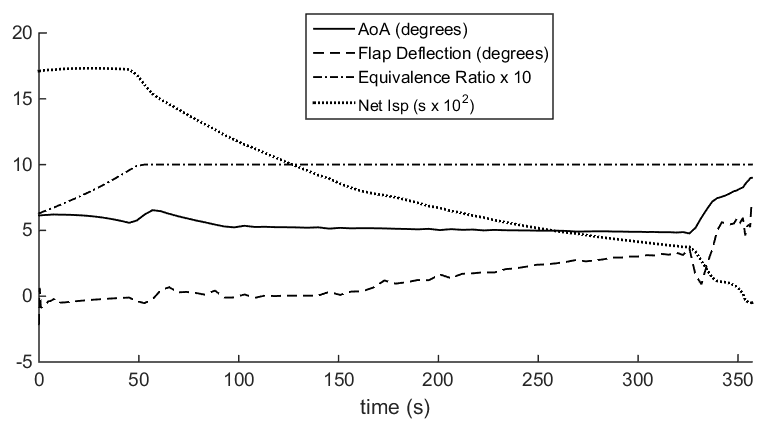
\includegraphics[width=0.8\linewidth]{figures/5_Ascent/qlimited-Vehicle}
\caption{}
\label{fig:qlimited-Vehicle}
\end{figure}

\subsection{Maximum Dynamic Pressure Variation}
\begin{figure}
\centering
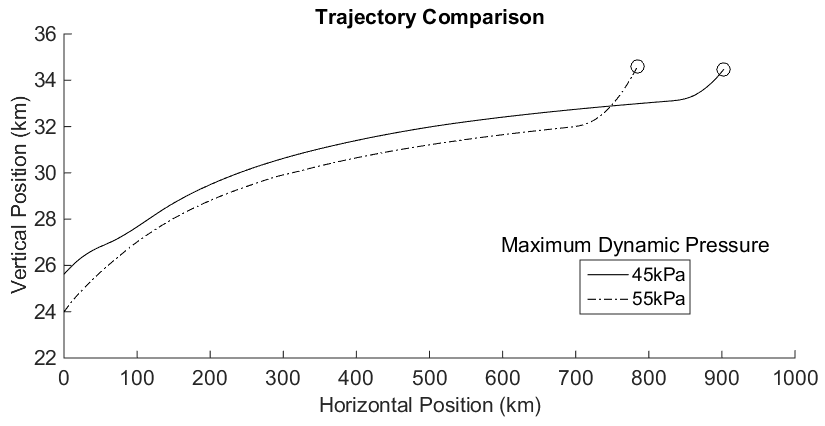
\includegraphics[width=0.9\linewidth]{figures/5_Ascent/Multipleq}
\caption{}
\label{fig:Multipleq}
\end{figure}
\begin{figure}
\centering
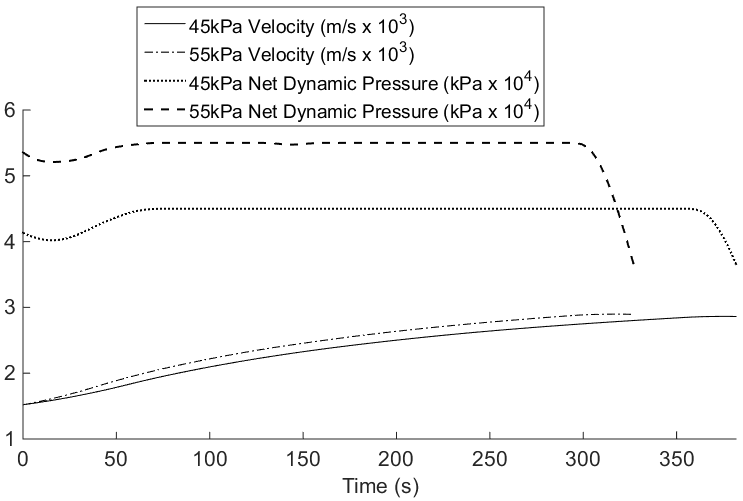
\includegraphics[width=0.8\linewidth]{figures/5_Ascent/MultipleqAero}
\caption{}
\label{fig:MultipleqAero}
\end{figure}
\begin{figure}
\centering
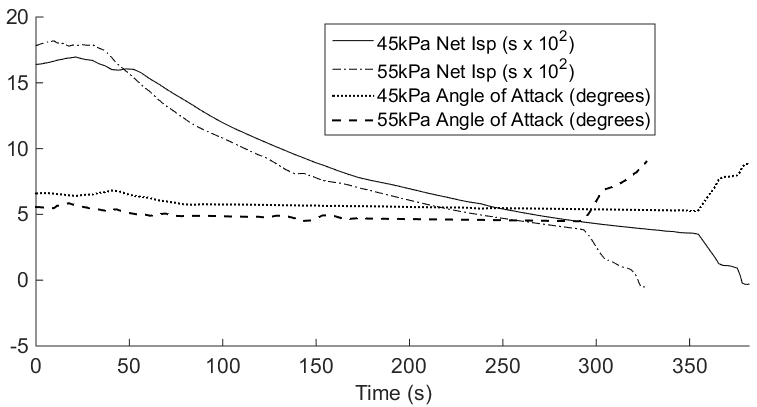
\includegraphics[width=0.8\linewidth]{figures/5_Ascent/Multipleq-Vehicle}
\caption{}
\label{fig:Multipleq-Vehicle}
\end{figure}

\subsection{Additional Drag Design Study}
\begin{figure}
\centering
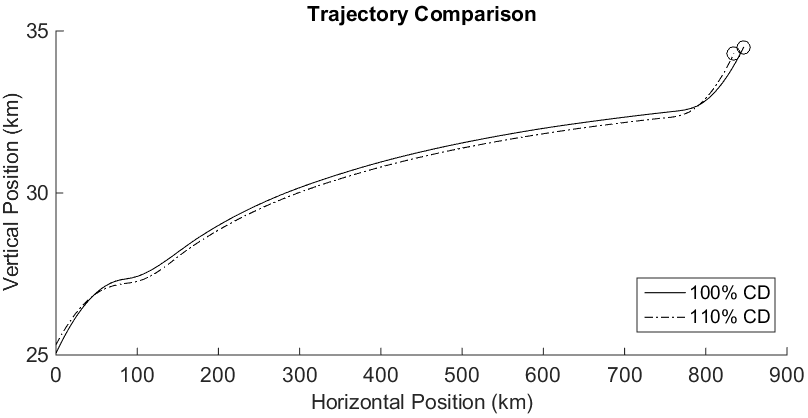
\includegraphics[width=0.9\linewidth]{figures/5_Ascent/DragComparisonTraj}
\caption{}
\label{fig:DragComparisonTraj}
\end{figure}
\begin{figure}
\centering
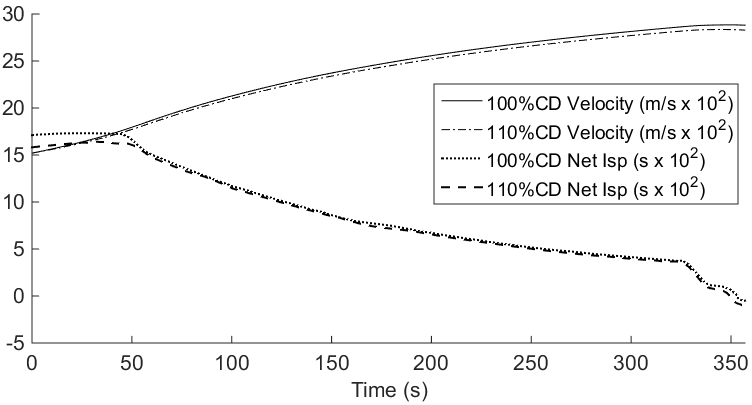
\includegraphics[width=0.8\linewidth]{figures/5_Ascent/DragComparisonOther}
\caption{}
\label{fig:DragComparisonOther}
\end{figure}

\section{First Stage Trajectory}
multiple release points
-fixed mass, optimal velocity
-fixed velocity, optimal mass


\begin{figure}
\centering
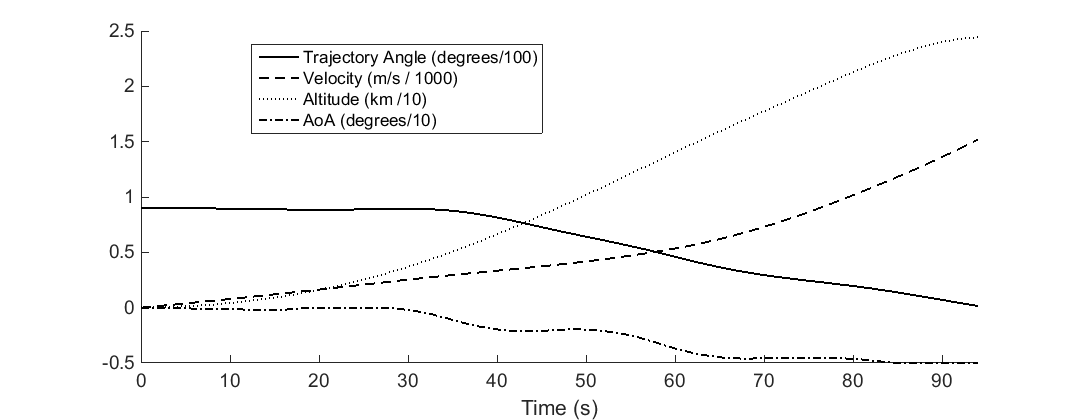
\includegraphics[width=1\linewidth]{figures/5_Ascent/FirstStage}
\caption{}
\label{fig:FirstStage}
\end{figure}


\section{Flyback trajectories }

-first stage to subsonic flight? 
-second stage
Abort analysis?